\chapter{Segmentation}
Segmentation is an importance process in computer vision, the goal of segmentation is to change the representation of an image into another way with more meaningful and easier to analyze. In another point of view, segmentation is process to assign the label to every pixel in an image to detect the pixels that have the same characteristics. The result of image segmentation is a set of distinct pixels with difference characteristics, or a set of contours extracted from the image.\\[0.2cm]
In computer vision, we have a lot of methods to segment an image. In the context of this chapter, we will mention the commonly method for segmentation. Besides, we also introduce the ways to record the information extracted from the contours of the image.
\section{Canny algorithm}
In 1986, \textbf{John F.Canny} had proposed a method to determine the edge in image. This is a technique to detect the useful structure of the object in digital image. Until now, the Canny algorithm\cite{canny1986computational} is used widely for the segmentation in computer vision. The process of Canny algorithm can be described in 4 steps as follows:
\begin{enumerate}
	\item Smoothing the image to reduce the noises by using Gaussian filter
	\item Finding the intensity and direction gradient of each pixel in image
	\item Eliminating the weak edge by using the edge thinning technique.
	\item Applying double threshold to determine the potential edges
\end{enumerate}
	\subsection{Gaussian filter}
	To smooth the image, a Gaussian filter is applied to convolve with the image. This step will help to reduce the effects of the noises on the edge detector. Normally, the equation of a Gaussian kernel with size $(2k+1)$ x $(2k + 1)$  is computed as:
	\begin{equation}
	H_{ij}=\frac{1}{2\pi\sigma^2}exp(-\frac{(i-(k+1))^2 + (j-(k+1))^2}{2\sigma^2});1\leq i,j \leq (2k+1)
	\end{equation}
	where $k$ is the size of kernel, and it should be a odd number.\\
	For example, a 3x3 Gaussian filter with $\sigma = 1 $ as followed:
	\begin{equation}
		G = 
		\begin{bmatrix}
		1 & 2 & 1\\
		2 & 4 & 2\\
		1 & 2 & 1		
		\end{bmatrix}
	\end{equation}	
	
	The selection of the size of the Gaussian kernel is important, it will affect the performance of the detector. If the size of the kernel is large, the detector can be sensitive to noise; otherwise, if the kernel's size is small, the detector can be destroy many strong edge. In the practice, this step is combined into Sobel convolution with a 3x3 kernel, which used to finding the intensity and direction gradients at each pixels of image.
	\subsection{Sobel convolution}
	The points belong to the edge in an image can stay in any direction, so the Canny algorithm uses four filters to detect the edges (vertical, horizontal and two diagonal edges) in the image. And the Sobel operator is used to detect the edges. This operator returns a value for the first derivative in horizontal direction $(G_x)$ and the vertical direction $(G_y)$. From these values, the gradient and direction of edge at each pixel are determined:
	\begin{equation}
		G = \sqrt{{G_x}^2 + {G_y}^2}
	\end{equation}
	\begin{equation}
		\phi = atan2(G_y,G_x)
	\end{equation}
	In this case, the kernel of Sobel convolution is 3x3, and it is also combined the Gaussian filter to smooth the image. The kernels are used to convolute the horizontal direction and vertical direction as follows:
	\begin{equation}
		G_x = 
		\begin{bmatrix}
		-1 & 0 & 1\\
		-2 & 0 & 2\\
		-1 & 0 & 1		
		\end{bmatrix}, 
		G_y = 
		\begin{bmatrix}
		-1 & -2 & -1\\
		0 & 0 & 0\\
		1 & 2 & 1		
		\end{bmatrix}
	\end{equation}
	
	The edge direction angle is rounded to one of four angles which were presented for four directions: vertical, horizontal, and two diagonals $0^o, 45^o, 90^o \text{ and } 135^o$.
	\subsection{Non-maximum suppression}
	Non-maximum suppression is applied to thin the edge in an image. Thus, this operation is used to suppress all the gradient values to 0 except the local maximal. At every pixel, it suppress the gradient value of the center pixels if its magnitude is smaller than the magnitude of one out of two neighbors in the gradient direction. In details:
	\begin{itemize}
	\item If the gradient direction angle is \textbf{0} degree, the point will be considered to be on the edge if the gradient magnitude is greater than the magnitude at pixels in the \textbf{east} and \textbf{west} directions.
	\item If the gradient direction angle is \textbf{45} degree, the point will be considered to be on the edge if the gradient magnitude is greater than the magnitude at pixels in the \textbf{north east} and \textbf{south west} directions.
	\item If the gradient direction angle is \textbf{90} degree, the point will be considered to be on the edge if the gradient magnitude is greater than the magnitude at pixels in the \textbf{north} and \textbf{south} directions.
	\item If the gradient direction angle is \textbf{135(-45)} degree, the point will be considered to be on the edge if the gradient magnitude is greater than the magnitude at pixels in the \textbf{north east} and \textbf{south west} directions.
	\end{itemize}
	\subsection{Double threshold}
	After applying the non-maximum suppression, the edges pixels are presented. However, there are still some edge pixels effected by noise. Double threshold will filter out the edge pixels with the weak gradient value and preserve the edge with the hight gradient value.
	\begin{itemize}
		\item A pixel called strong pixel (hence, it belong to the edge), if the edge pixel's gradient value is higher than the high threshold value.
		\item A pixel will be suppressed, if the edge pixel's gradient value is smaller than the low threshold value.
		\item A pixel called weak pixel (can be belong to the edge or not), if the edge pixel's gradient value is larger than low threshold value and smaller than high threshold value. A weak pixel can be belong to the edge if it connected with a strong pixel in 8-connected; else, it will be suppressed.
	\end{itemize}
	Thus, the accuracy of algorithm is depended on two parameters: the kernel of Gaussian filter and thresholds value. As said before, if we choose incorrect the kernel size of Gaussian filter, we can not reduce the noise or we can remove the real edge. Besides, the values of double threshold is also important to filter out the edge pixels. In practice, 1:3 is the good ratio between lower threshold  and upper threshold in Canny.
	\subsection{Summary}
	With applying double thresholding in the last stage, Canny had provied a strict condition to consider the weak edge as well as remove the pixels which were not belong to the edge. So far, Canny algorithm is good method to determined the edge in image, it is used by many application in image processing.
\section{Suzuki algorithm}
The Canny algorithm had detected the edge in the image. We can apply many difference methods to track the edge. \textbf{S. Suzuki} and \textbf{K. Abe}\cite{suzuki1985topological} had proprosed a method to get the border of object in image. This method is based on the topological structure analysis on binary image.\\[0.2cm]
Following this method, it detects two kinds of border in image. The first is outer border, which is defined by a set of border points between an arbitrary 1-component and the 0-component which surrounds it directly; another type is hole border which refers to the set of border points between a hole and the 1-componet which surrounds the hole directly. In this case, the 1-component (or 0-component) is connected component of 1-pixels (or 0-pixels).\\[0.2cm]
In our case, our purpose is getting the edges which were detectecd by Canny\cite{canny1986computational}. An edge is consider as an outer border or a hole border does not important. So, the Suzuki algorithm could make some changes to fit with our aim. The processes of algorithm is desribed as follows:\\[0.2cm]
Let an input binary image is \textbf{$F=\{f_{ij}\}$}. Set initially $NBD = 1$ (denoted the sequence number of border.)
\begin{enumerate}
	\item Select one of the following:
		\begin{enumerate}
			\item If \textbf{$f_{ij} = 1$} and \textbf{$f_{i,j-1} = 0$}, increment NBD, $(i_2,j_2) \gets (i,j-1)$ (pixel $(i,j)$ is the starting point of an outer border).
			\item If \textbf{$f_{ij} \geq 1$} and \textbf{$f_{i,j+1} = 0$}, increment NBD, $(i_2,j_2) \gets (i,j+1)$ (pixel $(i,j)$ is the starting point of an hole border).
			\item Otherwise, go to step (3)
		\end{enumerate}
	\item From the starting point \textbf{(i,j)}, the process to trace the edge is done by substeps following:
		\begin{itemize}
			\item[2.1] Starting from point $(i_2,j_2)$, look around clockwise the pixels in the neighborhood (8-connected) of $(i,j)$ and find the first non-zero pixel $(i_1,j_1)$. If no non-zero pixel is found, assign -NBD to $f_{ij}$ and go to step (3)
			\item[2.2] $(i_2,j_2) \gets (i_1,j_1)$ and $(i_3,j_3) \gets (i,j)$
			\item[2.3] Starting from the \textbf{next element of the pixel $(i_2,j_2)$} in the counterclock-wise order, check the pixels neighborhood of current pixel $(i_3,j_3)$ to find the first non-zero pixel $(i_4,j_4)$.
			\item[2.4] Chang the value $f_{i_3,j_3}$ of the pixel $(i_3,j_3)$ as follows:
				\begin{enumerate}
					\item If the pixels $(i_3,j_3+1)$ is a 0-pixel examined in the substep (2.3) then $f_{i_3,j_3} \gets -NBD$. Else, $f_{i_3,j_3} \gets NBD$ unless $(i_3,j_3)$ is on an already border.
					\item If the pixels $(i_3,j_3+1)$ is not a 0-pixel examined in the substep (2.3) and $f_{i_3,j_3} = 1$ then $f_{i_3,j_3} \gets NBD$
					\item Otherwise, do not change $f_{i_3,j_3}$.
				\end{enumerate}
			\item[2.5] If $(i_4,j_4) = (i,j)$ and $(i_3,j_3) = (i_1,j_1)$ (coming back to the starting point), then go to step (3); otherwise, $(i_2,j_2) \gets (i_3,j3), (i_3,j_3) \gets (i_4,j_4)$ and go back to step (2.3)
		\end{itemize}
	\item Resume the scan from the pixel $(i,j+1)$. The algorithm is stop when the scan reaches the lower right corner of the image.
\end{enumerate}
The obtained results from Suzuki algorithm are list of the edges of the object in the image. Each edge is list of connected points. This result is very important for the next steps of automatic detection landmarks.
\section{Approximated lines}
The list of points from Suzuki algorithm can used to present the object. But in some case to consider the feature of the object, the information from the list of points is not perfect. Instead of, we use another kind of the geometric object to represent the object. This is the line. In this section, we will describe the duration to get the approximated lines of object from the list of edge (each edge is represented by the list of points).\\[0.2cm]
The method is used to fragment the edge into a list of approximated line is a recursive algorithm\cite{thacker1995assessing}, which is a new improved version with the method proposed by Lowe\cite{lowe1987three} except the stop condition is considered as a parameter $\lambda$. The steps of algorithm are followed:
\begin{enumerate}
	\item Create a straight line $l$ between two endpoints of the edge
	\item Calculate the perpendicular distance from each point on edge to line $l$, and identifying the maximum point $p_m$.
	\item If the perpendicular distance from maximum point $p_m$ is greater than the stop condition($d(p_m,l) > \lambda$), then the edge is split at this point and both parts are reprocessed. Otherwise, if we do not have any $p_i$ that the perpendicular distance from they to $l$ greater than $\lambda$ then the edge can be represented by $l$. 
\end{enumerate}
\section{Pairwise Geometric Histogram}
In image processing, we have many techniques to describe the features of the image. With expect represent the image's features into the variant information for compare and representation, pairwise geometric histogram (PGH) method is chosen. PGH is constructed based on the geometry relative of the image's features. With an image is presented by the list of lines, the angle and perpendicular distance between two lines are importance characteristic to consider for re-constructor the image. Moreover, PGH is also fitwell when we apply some variants on the image such as translation or rotation because the angle and perpendicular distance between two lines are invariant. The process to calculate the PGH of an image which is represented by a list of lines as follows:
\begin{itemize}
	\item Choose arbitrary line as reference lines \textbf{$l_f$}
	\item For each other lines \textbf{$l$} in image, calculate the angle between \textbf{$l$} and \textbf{$l_f$}, and perpendicular distance from two endpoints of \textbf{$l$} to \textbf{$l_f$}.
	\item The process will stop when all line in the image are considered as reference line.
\end{itemize}
An importance note, during the process calculate the PGH, we need to keep the information of PGH to reconstruct the image or compare with other image.
\begin{figure}[h!]
\centering
\subfloat[The geometric relationship between two lines]{\label{fig:231}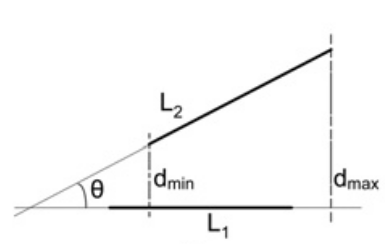
\includegraphics[width=0.4\textwidth]{./images/PGH_geo}}~~
\subfloat[The information of PGH is kept into a matrix]{\label{fig:232}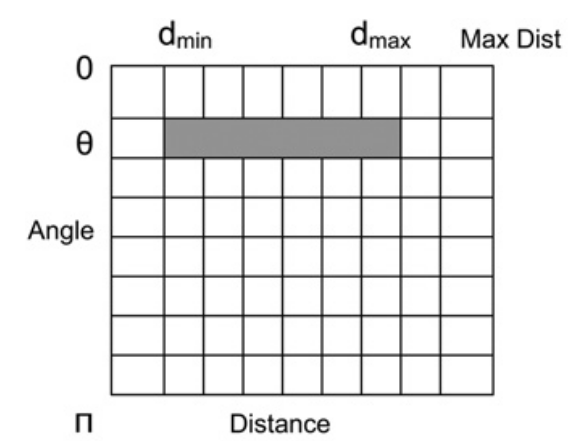
\includegraphics[width=0.4\textwidth]{./images/PGH}}
\caption{Example about geometric features and the pairwise geometric histogram}
\label{fig:figure_23}
\end{figure}~\\[0.2cm]
To detect the similarity between two images, we can use the pairwise geometric histogram matching via the similar distance of their probability distribution on histogram. The Bhattacharyya metric is common distance to compare two models. The form of Bhattacharyya is:
\begin{equation}
	\label{eq:1}
d_{Bhattacharyya} (H_{i}H_{j}) = \sum\limits_{\theta}^{\pi}\sum\limits_{d}^{d_{max}}\sqrt{H_{i}(\theta,d)H_{j}(\theta,d)}
\end{equation}
The significance of parameters in the formula \ref{eq:1}, as follows:
\begin{itemize}
\item $\theta$: angle value, range of $\theta$ in angle axis from 0 to $\pi$.
\item $d$: the perpendicular distance, range of $d$ in perpendicular distance from 0 to the maximum distance of arbitrary lines of shape.
\item $H_{i}(\theta,d)$ is an entry at row $\theta$ and column $d$ in PGH of image \textit{i}
\item $H_{j}(\theta,d)$ is an entry at row $\theta$ and column $d$ in PGH of image \textit{j}
\end{itemize}
\section{Bounding box detection}
In this section, we will discuss about the projection histogram technique which used to detect the distribution of pixels in many ways. Besides, we also mention the applying the projection histogram for detecting the bounding box around object in image.
\subsection{Projection histogram}
Projection histogram is one of the techniques that used to extract the feature of the image. The information of projection histogram was extracted from the distribution of the pixels on an arbitrary axis. In mathematics, a projection is a mapping of a set into a subset which is correspondence with its square for mapping composition. \\[0.2cm]
To find the projection histograms of a color image; we need to process on each channel color of the image and combine the result at the end of process. With a channel of image, we can create a lot of projection histogram i.e projection on x-axis, y-axis. The numer of the projection and the combining the projections are is depended on the goal of method. Figure \ref{fignprojection} decribes the x-axis projection and y-axis projection of an objection in the image.
\begin{figure}[h]
	\centering
	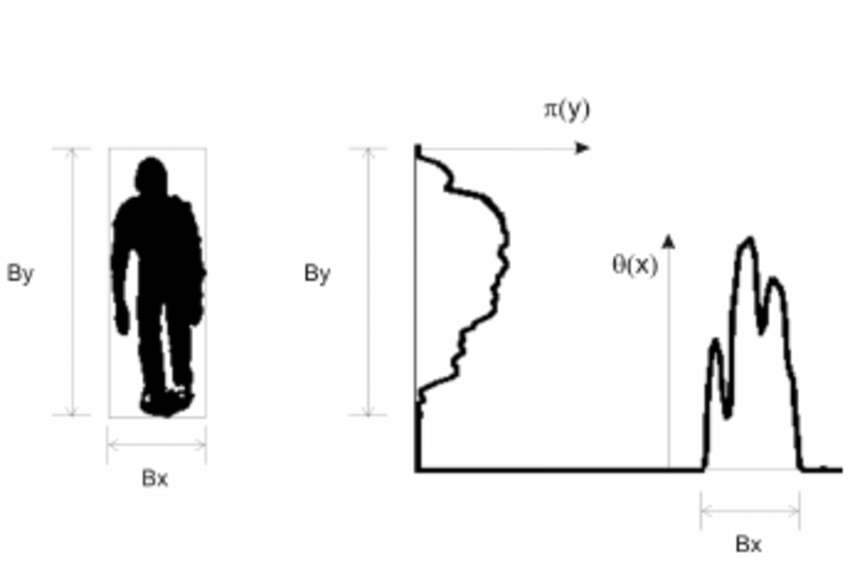
\includegraphics[scale=0.4]{images/projection}
	\caption{An example about projection histograms}
	\label{fignprojection}
\end{figure}
\subsection{Bounding box}
The bounding box of insect in the image is result by applying some analysis on the projection histograms. Actually, to determine the postion of bounding box that we just need to indicate the position of two (or four) corners ((top-left, bottom-right)or (top-left, top-right, bottom-left, bottom-right) of the box.\\[0.2cm]
The information of these corners was determined by analysis the horizontal projection and vertical projection of the image. The analysis to indicate the left and right border of the peak region on each projection. The steps in the method are used to find the bounding box of object in image as followed:
\begin{itemize}
	\item Quantize the image to N colors (can be decrease the number of bit to store)
	\item Detect the horizontal and vertical projection of the image
	\item The corners are indicating by the intersection of the borders between horizontal and vertical projection.
\end{itemize}
\section{Texture segmentation}
